\documentclass[18pt]{article}
\usepackage[utf8]{inputenc}
\usepackage[T1]{fontenc}
\usepackage{ragged2e}
\usepackage{caladea}
\usepackage{graphicx}
\usepackage{longtable}
\usepackage{wrapfig}
\usepackage{rotating}
\usepackage{epigraph}
\usepackage[normalem]{ulem}
\usepackage{hyperref}
\usepackage{amsmath}
\usepackage{amssymb}
\usepackage{capt-of}
\usepackage{hyperref}
\usepackage{fancyhdr}

\title{
 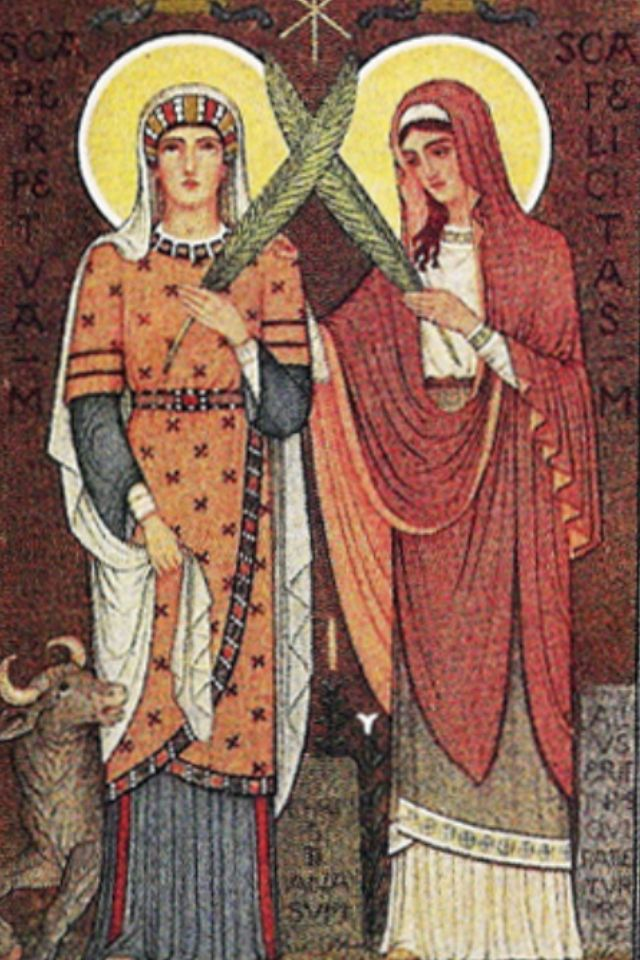
\includegraphics[scale=.45, trim={10cm, 0, 10cm, 0}]{./assets/imagem.jpg}
  \par
   NOVENA A Santas Felicidade e Perpétua}
  \date{Data Litúrgica: 07/03}

% Comando para fazer "Sumário" não aparecer no Sumário.
\renewcommand{\contentsname}{Sumário}
\begin{document}
\maketitle

\thispagestyle{empty} %zera a primeira página

\pagestyle{fancy}
\fancyhf{} % clear existing header/footer entries
\fancyfoot[LO, CE]{

\includegraphics[scale=0.2]{./assets/cross.png} Santas Felicidade e Perpétua, rogai por nós!
}
% Place Page X of Y on the right-hand
% side of the footer
\fancyfoot[R]{\thepage}

\newpage

\tableofcontents

\centering
\vfill
Visite-nos no Telegram: \url{https://t.me/CotidieNovena}
\newpage

\newpage


%%%%%%%%%%%%%%%%%%%%%%%%%%%%%%%%%%%%% História %%%%%%%%%%%%%%%%%%%%%%%%%%%%%%%%%%%%%%%%%%%

\begin{justify}

 \begin{center}
  \section{História}\label{sec:História} % (fold)
 \end{center}





  \begin{justify}
  \subsection{Origem}
 \end{justify}

Muitas mulheres, jovens, mães, foram martirizadas no ano 203, em Cartago (norte da África, atual cidade de Túnis). Dentre elas, Perpétua, que tinha aproximadamente 22 anos. Era nobre de família rica, sendo seu pai o único da família a ser pagão. Quando foi levada para a prisão, tinha um filho recém-nascido. Felicidade era escrava de Perpétua e, quando foi para a prisão, estava com oito meses de gestação e deu à luz uma menina neste lugar.


 \begin{justify}
 \subsection{O cárcere}
 \end{justify}

Elas foram presas por causa de um decreto do imperador romano, Lúcio Septímo Severo, que condenaria à morte aqueles que se considerassem cristãos. Em seus escritos, Perpétua narra: “Nos jogaram no cárcere e eu fiquei consternada, porque nunca tinha estado em um lugar tão escuro. O calor era insuportável e éramos muitas pessoas em um subterrâneo muito estreito. Parecia que ia morrer de calor e de asfixia, e sofria por não poder ter, junto a mim, o meu filho, que era de tão poucos meses e necessitava muito de mim. O que eu mais pedia a Deus era a graça para ser capaz de sofrer e lutar por nossa santa religião”.

Foi na prisão também que as companheiras, pelo batismo, oficializaram a pertença delas a Deus. Ainda na prisão, Perpétua escreve, em um diário, as atrocidades que viveu naquele lugar, ressaltando a sua coragem e amor a Cristo. Esse diário é considerado um dos textos cristãos mais antigos, ele é conhecido hoje como: a Paixão das Santas Perpétua e Felicidade (em Latim: Passio sanctarum Perpetuae et Felicitatis).

\vspace{0.7cm}

 \begin{justify}
 \subsection{Martírio}
 \end{justify}

As duas foram lançadas na arena juntamente com outros companheiros para serem pisoteadas por touros e vacas. Perpétua foi a primeira a ser atingida. Felicidade a ergueu do chão, ficando lado a lado, dando força uma a outra e demonstrando coragem, que é própria dos mártires. Perpétua animou o grupo com estas palavras: “Fiquem firmes na fé e amem-se uns aos outros, todos vocês! Não deixem que o martírio seja pedra de tropeço para vocês.”


Felicidade foi a primeira a ser degolada. Em seguida, o soldado, que faria o mesmo com Perpétua, errou o local do golpe, fazendo com que ela lançasse um grito de dor, mas, com sua mão, ela indicou, ao seu algoz, o local a ser cortado pelo machado dele.

\vfill

\begin{center}
 \href{https://santo.cancaonova.com/santo/santas-perpetua-e-felicidade/}{Fonte: Canção Nova}
\end{center}

%%%%%%%%%%%%%%%%%%%%%%%%%%%%%%%%%%%%% Orações %%%%%%%%%%%%%%%%%%%%%%%%%%%%%%%%%%%%%%%%%%%

\newpage
\begin{center}
 \section{Orações}\label{sec:Orações} % (fold)
\textit{Em nome do Pai, e do Filho, e do Espírito Santo. Amém.}
\end{center}

\subsection{Oração Incial}\label{sec:Oração_Inicial} % (fold)

Ó Deus, que, movido pelo amor, fez com que os Santos Mártires Perpétua e Felicidade desafiassem seus perseguidores e superassem o tormento da morte, conceda-nos, pedimos, por suas orações, que possamos sempre crescer em seu amor.

Por nosso Senhor Jesus Cristo, seu Filho, que vive e reina com você na unidade do Espírito Santo, um só Deus, para sempre. Amém.

Você os coroou com glória e honra, ó Senhor.  
E os colocou sobre as obras de suas mãos.

Conceda-nos, suplicamos, ó Senhor nosso Deus, que possamos venerar com devoção incessante os triunfos de seus santos Mártires, Perpétua e Felicidade; e embora não possamos prestar-lhes a honra que é devida, que ao menos possamos apresentar-lhes nossa humilde homenagem.

Amém.



\subsection{Oração Final}\label{sec:Oração_Final} % (fold)
\begin{center}
\textbf{Pai Nosso, Ave Maria, Glória ao Pai.}


\vfill
\subsection*{Créditos:}
\href{https://catholicnovenaapp.com/novenas/sts-perpetua-and-felicity-novena/#day-1-prayer}{Catholic Novena App}

\end{center}


\end{justify}

\end{document}
